\documentclass[standalone]{beamer}

\begin{document}
\section{Aliens 優化}

\begin{frame}{\btitle{前言}}
  \begin{itemize}
    \item Aliens 優化又稱 WQS 二分搜,據說在很久之前就在大陸被發明了
    \item 在台灣也會被稱為「帶感情 DP」
    \item 不過使它發揚光大的是 IOI 2016 一道名為 Aliens 的題目
    \item 近幾年基於一些不明的原因開始在臺灣競程界流行了起來,所以在這邊簡單的介紹一下
  \end{itemize}
\end{frame}

\begin{frame}{\btitle{例題}}
  \begin{problem}
    給定一棵 $N$ 個節點的帶權樹以及一個常數 $K$,請找出 $K$ 條邊使得邊權總和最大且不存在兩條邊有共同頂點。

    % $(N \leq 2.5 \times 10^5, K \leq N - 1)$
    \begin{itemize}
      \item $N \leq 2.5 \times 10^5$
      \item $K \leq N - 1$
    \end{itemize}
  \end{problem}
\end{frame}

\begin{frame}{\btitle{例題}}
  先考慮沒有 $K$ 這個限制下要怎麼處理,也就是說找出一些邊使得邊權總和最大且沒有共端點
  
  這是一個經典在樹上 DP 的題目:令(為了方便,定義一個點被選了就是有一條相鄰的邊被選了)

  \begin{align*}
    dp(v, 0) &\coloneqq \text{$v$ 的子樹在 $v$ 還沒有被選的情況下的最大答案} \\
    dp(v, 1) &\coloneqq \text{$v$ 的子樹在 $v$ 被選的情況下的最大答案} \\
  \end{align*} 
\end{frame}

\begin{frame}{\btitle{例題}}
  \begin{itemize}
  % \begin{equation}
    \item $dp(v, 0) = \sum_{(u, w) \in G(v)}\max(dp(u, 0), dp(u, 1))$
    % \end{equation}

    % \begin{equation}
    \item $dp(v, 1) = \max_{(u, w) \in G(v)} \{dp(u, 0) + w +$ $ 
      \sum_{(u^\prime, w^\prime) \in G(v), u^\prime \neq u}\max(dp(u^\prime, 0), dp(u^\prime, 1)) \}$
    % \end{equation}

    \item 其中式子一代表不取 $v$ 向下延伸的邊的 case,所以並不在乎小孩有沒有被選到。而式子二則是枚舉要取哪條邊,所以對應的小孩一定不能被選到,而其他則無所謂。透過一些預處理可以使得這個 DP 算法的複雜度壓到 $O(N)$
    \item 那要怎麼處理有限制個數的狀況呢?其中一個方法是在 DP 狀態多記一個維度代表取了幾條邊,不過會使得複雜度變成至少 $O(NK)$,並不是一個足夠有效率的方法
  \end{itemize}
\end{frame}

\begin{frame}{\btitle{性質}}
  \begin{itemize}
    \item 我們需要以下的性質來幫助解題
    \begin{theorem}[性質]
      令 $f(K)$ 為恰取 $K$ 條邊的最大邊權總和,則 $f$ 是一個凹函數(concave function)\footnote{為了方便說明,這邊指的 concave function 都只定義在整數上面。}。亦即,這個函數滿足 $f(K + 1) - f(K) \leq f(K) - f(K - 1)$。
    \end{theorem}
    \item 也就是 $f$ 的差分遞減。再白話一點的話,就是取第 $K + 1$ 條邊的\textbf{淨獲益}不會比取第 $K$ 條邊的淨獲益來得高(也就是說,隨著 $K$ 的值越來越大,賺到的會越來越少)
    \item 有了這個性質以後,原本的問題就可以被轉為下面的問題
  \end{itemize}
\end{frame}

\begin{frame}{\btitle{性質}}
  \begin{itemize}
    \item 
    \begin{problem}[等價的問題]
      現在有一個凹函數 $f$,我們想知道 $f(K)$ 的值是多少。可惜的是,沒有好的演算法可以直接計算 $f(K)$,可以知道的只有給定 $p$,$f(x) - px$ 的最大值以及最大值發生的位置。要如何運用這些資訊求出 $f(K)$ 呢?
    \end{problem}
    \item 先暫停一下,在給定 $p$ 的情況下,要怎麼算出 $f(x) - px$ 呢?
    \item 如果有一條邊被選擇,我們就額外的扣掉 $p$ 這個邊權
  \end{itemize}
\end{frame}

\begin{frame}{\btitle{性質}}
  \begin{problem}[等價的問題]
    現在有一個凹函數 $f$,我們想知道 $f(K)$ 的值是多少。可惜的是,沒有好的演算法可以直接計算 $f(K)$,可以知道的只有給定 $p$,$f(x) - px$ 的最大值以及最大值發生的位置。要如何運用這些資訊求出 $f(K)$ 呢?
  \end{problem}

  令 $M(p)$ 為 $f(x) - px$ 的最大值,$V(p)$ 為最大值發生的位置,若有多個最大值,則定義為 $x$ 值最小的那個最大值

  不難發現,假設現在我們幸運的找到了一個 $p$,使得 $V(p) = K$,那麼 $f(K)$ 就可以直接用 $f(K) = M(p) + pK$ 算出來了,所以我們的目標就是快速找到這樣的 $p$
\end{frame}

\begin{frame}{\btitle{性質}}
  \begin{itemize}
    \item 令 $M(p)$ 為 $f(x) - px$ 的最大值,$V(p)$ 為最大值發生的位置,若有多個最大值,則定義為 $x$ 值最小的那個最大值
    \item 不妨把 $f(x)$ 的圖形在二維平面上畫出來
    \item 觀察一下後可以知道,$f$ 的長相會長得像一個\textbf{上凸包},且 $V(p) = x$ 就代表存在一條斜率為 $p$ 的直線與 $f$ 的圖形相切於 $(x, f(x))$
    \item 原因是一條斜率為 $p$ 的直線切在 $x$ 上就代表通過 $x$ 這點且斜率為 $p$ 的直線的截距是所有點中最大的
    \item 令切線為 $g(x) = px + b$,則帶入 $(x, f(x))$ 後得到截距 $b = f(x) - px$,恰好與 $M(p)$ 的定義吻合
    \item 不僅如此,當 $x$ 越大時,切在 $(x, f(x))$ 的切線斜率是遞減的。這就告訴我們其實我們可以透過二分搜 $p$ 來找到 $V(p) = K$,再藉此推算 $f(K)$ 
  \end{itemize}
\end{frame}

\begin{frame}{\btitle{性質}}
  \begin{figure}[H]
  \centering
  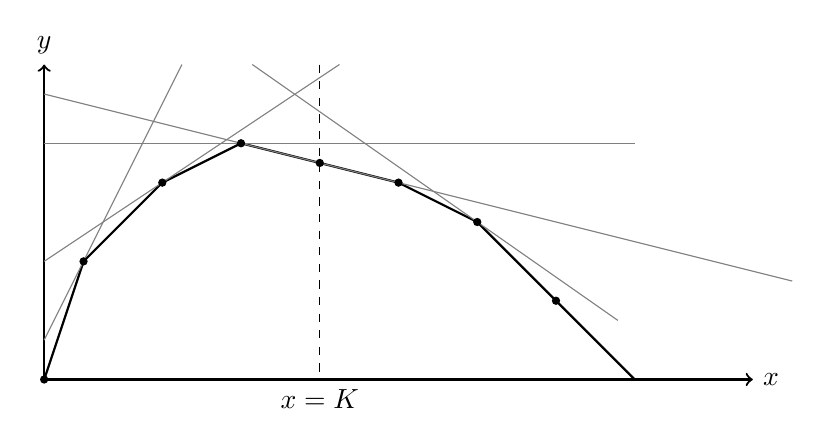
\begin{tikzpicture}[scale=0.5]
      % Draw axes
      \draw [<->,thick] (0,8) node (yaxis) [above] {$y$}
          |- (18,0) node (xaxis) [right] {$x$};
      \coordinate (f0) at (0, 0);
      \coordinate (f1) at (1, 3);
      \coordinate (f2) at (3, 5);
      \coordinate (f3) at (5, 6);
      \coordinate (f4) at (7, 5.5);
      \coordinate (f5) at (9, 5);
      \coordinate (f6) at (11, 4);
      \coordinate (f7) at (13, 2);
      \coordinate (f8) at (15, 0);

      \draw [thick] (f0) -- (f1);
      \draw [thick] (f1) -- (f2);
      \draw [thick] (f2) -- (f3);
      \draw [thick] (f3) -- (f4);
      \draw [thick] (f4) -- (f5);
      \draw [thick] (f5) -- (f6);
      \draw [thick] (f6) -- (f7);
      \draw [thick] (f7) -- (f8);
      \draw [domain=1:8,smooth,variable=\y,gray] plot ({0.5 * (\y - 1)}, {\y});
      \draw [domain=3:8,smooth,variable=\y,gray] plot ({(\y - 3) * 1.5}, {\y});
      \draw [domain=0:15,smooth,variable=\x,gray] plot ({\x}, {6});
      \draw [domain=2.5:7.25,smooth,variable=\y,gray] plot ({-4 * \y + 29}, {\y});
      \draw [domain=1.5:8,smooth,variable=\y,gray] plot ({(\y - 11.7) / -0.7}, {\y});
      \node at (7, -0.5) (xk) {$x = K$};
      \draw [dashed] (7, 8) -- (7, 0);
      \fill (f0) circle (3pt);
      \fill (f1) circle (3pt);
      \fill (f2) circle (3pt);
      \fill (f3) circle (3pt);
      \fill (f4) circle (3pt);
      \fill (f5) circle (3pt);
      \fill (f6) circle (3pt);
      \fill (f7) circle (3pt);
  \end{tikzpicture}
  \caption{一個可能的 $f(x)$ 以及切線們。注意到切線斜率隨著 $x$ 遞增而遞減,且 $f(x)$ 在 $x = K$ 之處等差。}
  \end{figure}
\end{frame}

\begin{frame}{\btitle{性質}}
  \begin{itemize}
    \item 這邊其實有一個問題,那就是我們可以透過二分搜找到最小的 $p$ 使得 $V(p) \leq k$,但這不保證就真的有那麼一個 $p$ 使得 $V(p) = k$
    \item 不過這件事只會發生在當 $f$ 在 $K \in [V(p), V(p + 1)]$ 之間是等差的情形
    \item 所以一個解決方法是分別求出 $f(V(p))$ 與 $f(V(p + 1))$ 之後內插得到 $f(K)$,也就是說 $f(K) = f(V(p)) + \frac{f(V(p + 1)) - f(V(p))}{V(p + 1) - V(p)}\left(K - V(p)\right)$
\end{itemize}
\end{frame}
\begin{frame}{\btitle{性質}}
\begin{itemize}
    \item 另一種不需要內插的做法用到了 $V(p)$ 定義為最小的最大值發生點以及我們找到的是最小滿足條件的 $p$,在這個情況下,由於 $f(x) - px$ 的頂部是平的,所以我們會有 $f(V(p)) - pV(p) = M(p) = f(K) - pK \implies f(K) = M(p) + pK$
    \item 因此只要找到 $M(p)$ 之後便可以直接找出 $f(K)$ 的值
    \item 一般來說,遇到的題目大部分的 $f$ 都是整數到整數的函數,在這個情況底下 $f$ 形成的凸包的斜率也都會是整數,所以上面講的二分搜以及內插全部都可以在整數上完成,比起使用浮點數計算,在效率以及誤差上會有很大的提升
    \item 另外,這邊並沒有講到合理的二分搜上下界要定在哪,這部分請讀者自行推導一下
  \end{itemize}
\end{frame}

\begin{frame}{\btitle{性質}}
\begin{figure}[H]
\centering
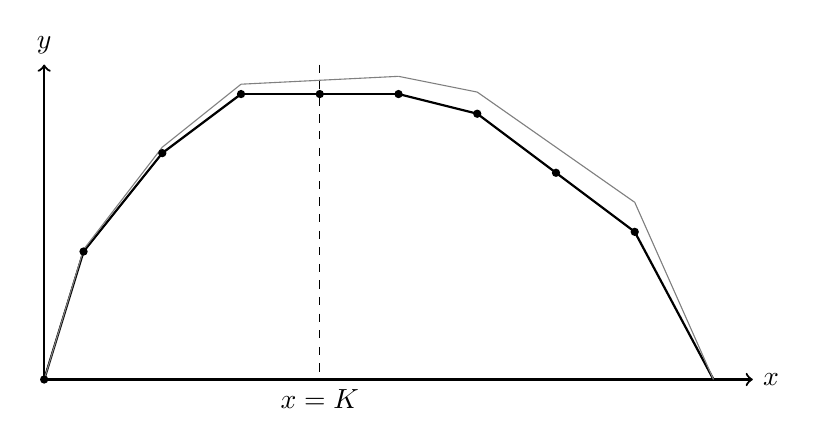
\begin{tikzpicture}[scale=0.5]
    \draw [<->,thick] (0,8) node (yaxis) [above] {$y$}
        |- (18,0) node (xaxis) [right] {$x$};
    \coordinate (f0) at (0, 0);
    \coordinate (f1) at (1, 3.25);
    \coordinate (f2) at (3, 5.75);
    \coordinate (f3) at (5, 7.25);
    \coordinate (f4) at (7, 7.25);
    \coordinate (f5) at (9, 7.25);
    \coordinate (f6) at (11, 6.75);
    \coordinate (f7) at (13, 5.25);
    \coordinate (f8) at (15, 3.75);
    \coordinate (f9) at (17, 0);

    \coordinate (g0) at (0, 0);
    \coordinate (g1) at (1, 3.3);
    \coordinate (g2) at (3, 5.9);
    \coordinate (g3) at (5, 7.5);
    \coordinate (g4) at (7, 7.6);
    \coordinate (g5) at (9, 7.7);
    \coordinate (g6) at (11, 7.3);
    \coordinate (g7) at (13, 5.9);
    \coordinate (g8) at (15, 4.5);
    \coordinate (g9) at (17, 0);

    \draw [thick] (f0) -- (f1);
    \draw [thick] (f1) -- (f2);
    \draw [thick] (f2) -- (f3);
    \draw [thick] (f3) -- (f4);
    \draw [thick] (f4) -- (f5);
    \draw [thick] (f5) -- (f6);
    \draw [thick] (f6) -- (f7);
    \draw [thick] (f7) -- (f8);
    \draw [thick] (f8) -- (f9);

    \draw [gray] (g0) -- (g1);
    \draw [gray] (g1) -- (g2);
    \draw [gray] (g2) -- (g3);
    \draw [gray] (g3) -- (g4);
    \draw [gray] (g4) -- (g5);
    \draw [gray] (g5) -- (g6);
    \draw [gray] (g6) -- (g7);
    \draw [gray] (g7) -- (g8);
    \draw [gray] (g8) -- (g9);

    \node at (7, -0.5) (xk) {$x = K$};
    \draw [dashed] (7, 8) -- (7, 0);

    \fill (f0) circle (3pt);
    \fill (f1) circle (3pt);
    \fill (f2) circle (3pt);
    \fill (f3) circle (3pt);
    \fill (f4) circle (3pt);
    \fill (f5) circle (3pt);
    \fill (f6) circle (3pt);
    \fill (f7) circle (3pt);
    \fill (f8) circle (3pt);
   
\end{tikzpicture}
\caption{$f(x) - px$ 的圖形,其中 $p$ 為最小的 $p$ 使得 $V(p) \leq K$。$x = K$ 之處變為平的。注意到如果二分搜的方向反了(找最大的 $p$ 使得 $V(p) \geq K$ )且 $V(p)$ 的定義不變的話,$f(x) - px$ 會變成淺色的樣子,$x = K$ 的地方就不是平的,直接推 $f(K)$ 便會出錯。}
\end{figure}
\end{frame}

\begin{frame}{\btitle{性質}}
  \begin{itemize}
    \item 回到原題,由於我們已經證明了這題的 $f(x)$ 是凹函數,所以可以套用 Aliens 優化
    \item 而一開始提到的 DP 可以很輕易的被修改成計算 $f(x) - px$ 最大值的形式,只要在取邊相對應的轉移式那邊多扣 $p$ 即可
    \item 至此,我們已經把原本看似高維的問題轉為了一維的問題,而這也是 Aliens 優化最常被使用的地方
    \item 最後要提到的是,大部分的情況下,題目中函數的凹性證明並不會像例題那樣簡單
    \item 據說 IOI 官方也沒有給 Aliens 的證明。所以大部分的時候都是靠感覺,或是本機寫暴力對拍跑跑看小 case 來確認性質
    \item 另外,由於凸函數(convex function)就是凹函數取負,所以上述的所有推導在差分遞增的情況也都成立,修改細節留給讀者自行練習
  \end{itemize}
\end{frame}

\begin{frame}
  感謝大家的聆聽~
\end{frame}

\end{document}
